\subsection{Event-Driven Architecture}

An \definition{Event-Driven Architecture} uses \textbf{events to trigger and communicate between decoupled services} and is common in modern applications built with microservices. An event is a change in state, or an update, like an item being placed in a shopping cart on an e-commerce website. Events can either carry the state (the item purchased, its price, and a delivery address) or events can be identifiers (a notification that an order was shipped).

Often it's called \textbf{publish-subscribe} (publish is the event generation, and subscribe is the declaration of the interest).

\begin{flushleft}
    \textcolor{Green3}{\textbf{\faIcon{check} Benefits}}
\end{flushleft}
\begin{itemize}
    \item \textbf{Very common in modern development practices} (e.g. continuous integration and deployment, such as GitHub Actions).

    \item \textbf{Easy addition/deletion of components} (publishers and subscribers are decoupled; the event dispatcher handles this dynamic set).
\end{itemize}

\begin{flushleft}
    \textcolor{Red2}{\textbf{\faIcon{exclamation-triangle} Problems}}
\end{flushleft}
\begin{itemize}
    \item \textbf{Potential scalability problems} (the event dispatcher may become a bottleneck under high workload).
    
    \item \textbf{Ordering of events} (not guaranteed, not straightforward).
\end{itemize}

\highspace
Other characteristics of this architecture:
\begin{itemize}
    \item THe messages and the events are \textbf{asynchronous}.
    
    \item Computation is \textbf{reactive} (driven by receipt of message).

    \item \textbf{Destination} of messages \textbf{determined by receiver}, not sender (location/identity abstraction).

    \item \textbf{Loose coupling} (senders and receivers added without reconfiguration).
    
    \item \textbf{Flexible} communication means (one-to-many, many-to-one, many-to-many).
\end{itemize}
Some \example{examples} of relevant technologies are: \href{https://kafka.apache.org/}{Apache Kafka} and \href{https://www.rabbitmq.com/}{RabbitMQ}.

\newpage

\subsubsection{Apache Kafka}

\definition{Kafka} is a \textbf{framework} for the event-driven paradigm:
\begin{itemize}
    \item Includes primitives to create \textbf{event produces} and \textbf{consumers} and a runtime infrastructure to handle \textbf{event transfer} from producers to consumers.
    
    \item \textbf{Stores events} durably and reliably.
    
    \item Allow consumers to \textbf{process events} as they occur or retrospectively.
\end{itemize}
These services are offered in a distributed, highly scalable, elastic, fault-tolerant, and secure manner.

\begin{figure}[!htp]
    \centering
    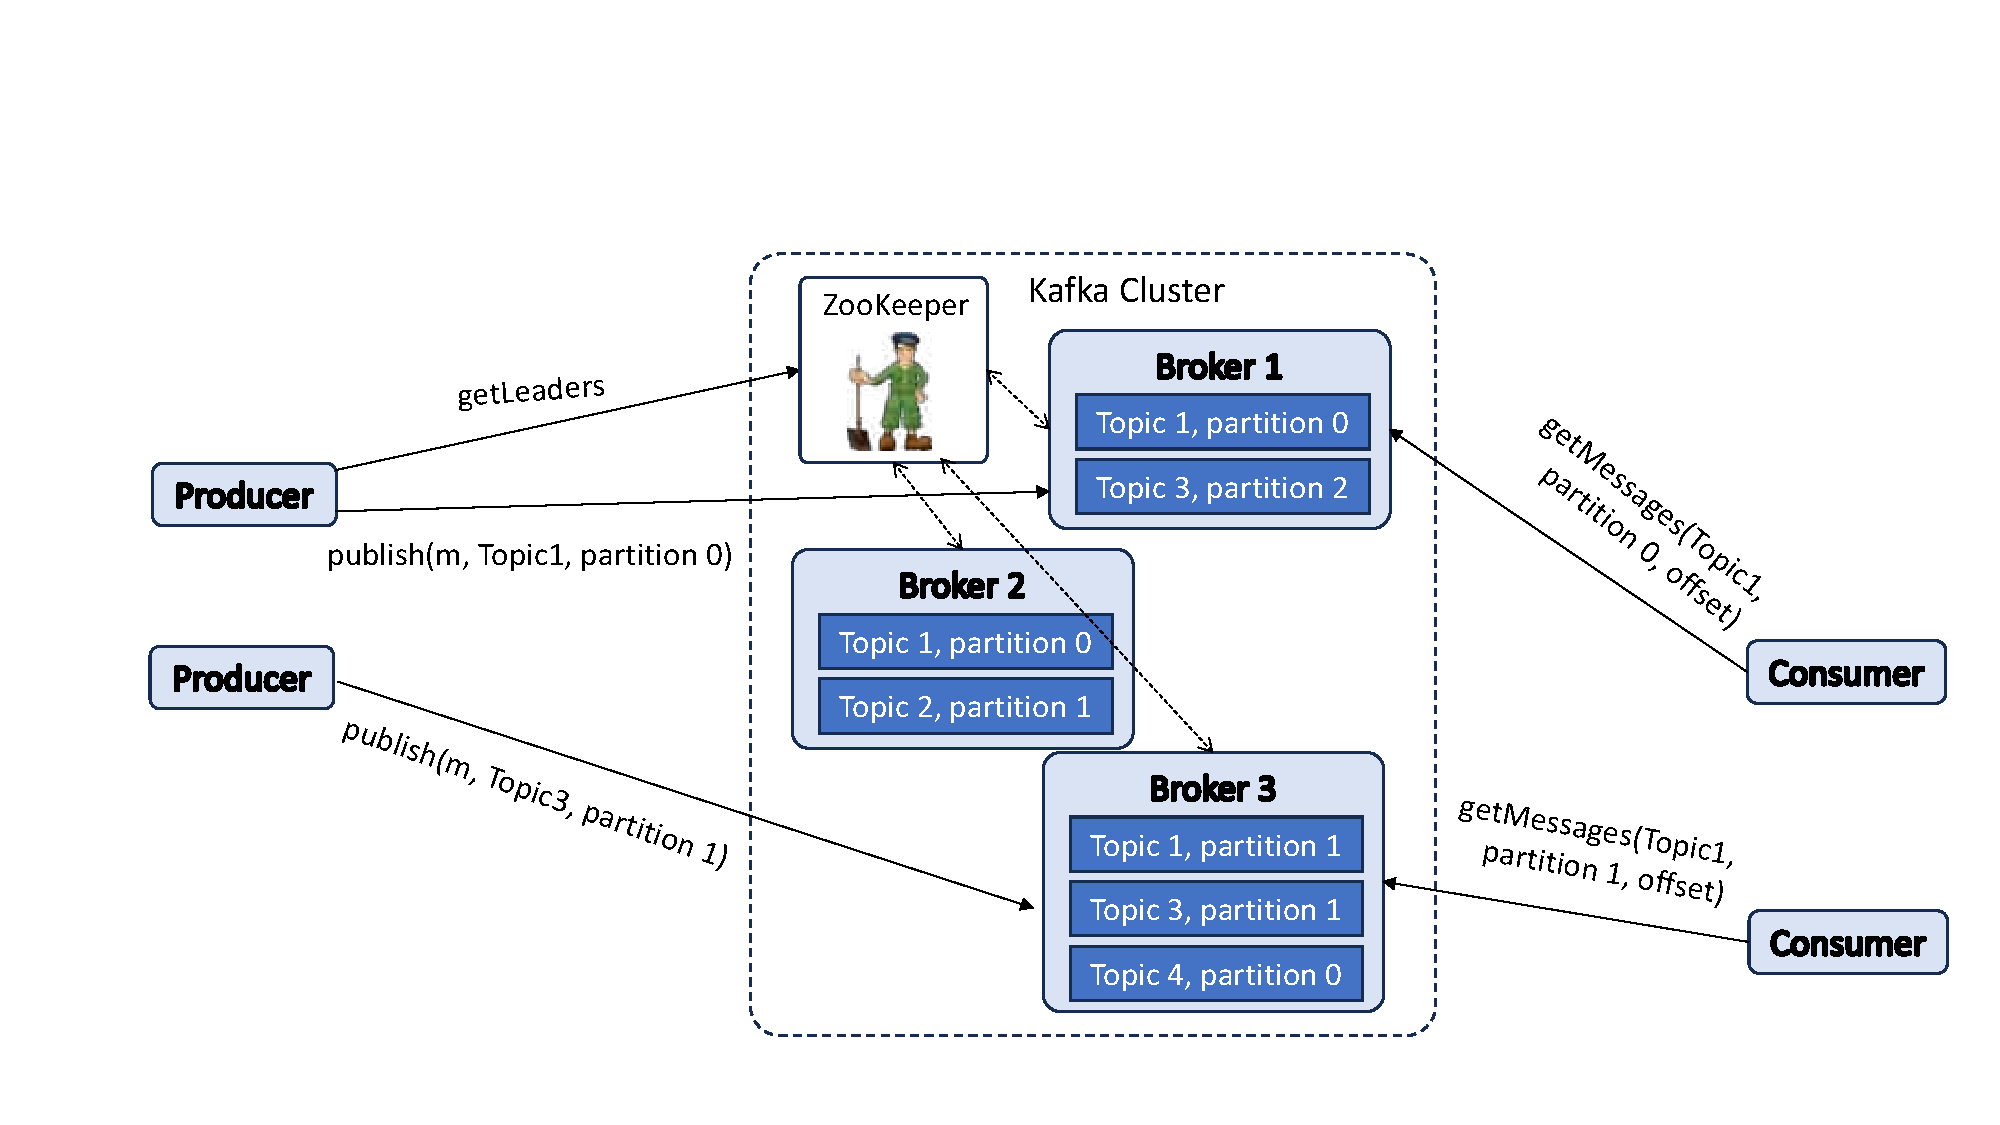
\includegraphics[width=\textwidth]{img/kafka-arch-1.pdf}
    \caption{Kafka architecture (the ZooKeeper is a \dquotes{health manager}).}
\end{figure}

\noindent
Some important features:
\begin{itemize}
    \item Each \textbf{broker} handles a set of \textbf{topics} and \textbf{topic partitions}, parts including sets of messages on the topic.

    \item The \emph{partitions} are independent from each other and can be \textbf{replicated} on multiple brokers for fault tolerance.

    \item There is \textbf{one leading broker per partition}. The other brokers containing the same partition are \textbf{followers}.
    
    \item The \textbf{producers} know the available leading brokers and send messages to them.
    
    \item \textbf{Messages in the same topic} are organized in \textbf{batches} at the producers' side and then sent to the broker when the batch size overcomes a certain threshold.

    \item \textbf{Consumers} adopt a \textbf{pull approach}. They \emph{receive in a single batch all messages} belonging to a certain partition starting from a specified offset.

    \item \textbf{Messages} remain \textbf{available} at the brokers' side \textbf{for a specified period} and can be \textbf{read multiple times} in this period.
    
    \item The leader keeps track of the \textbf{in-synch followers}.
    
    \item \textbf{ZooKeeper is used to monitor the correct operation of the cluster}. All brokers send heartbeats to ZooKeeper. ZooKeeper will replace a failed broker by electing a new leader for all partitions that the failed broker was leading. It can also start/restart brokers.
\end{itemize}

\begin{center}
    \large
    \textcolor{Red2}{\textbf{Message delivery}}
\end{center}

\begin{flushleft}
    \textcolor{Red2}{\textbf{Producer}}
\end{flushleft}
\begin{enumerate}
    \item Brokers commit messages by storing them in the corresponding partition;
    
    \item Leader adds the message to followers (replicas) if available.
\end{enumerate}

\begin{figure}[!htp]
    \centering
    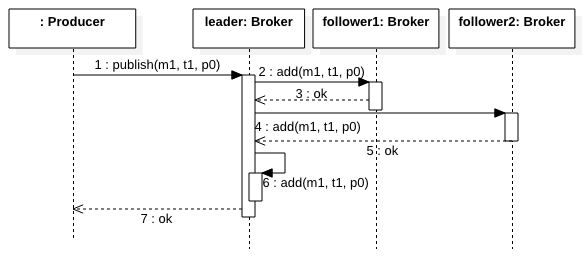
\includegraphics[width=\textwidth]{img/kafka-producer.png}
    \caption{Sequence diagram Kafka producer.}
\end{figure}

\noindent
A possible \textbf{issue}: in case of failure, the \textbf{producer may not get the response} (message number 7 in figure). In this case, the producer has to resend the message and kafka brokers can identify and eliminate duplicates.

\highspace
Synchronization with replicas can be transactional and it's possible to choose between the following options:
\begin{itemize}
    \item \textbf{Exactly-once} semantics is possible but long waiting time. So \textbf{replicas are not allowed}, but the problem is that Kafka spent a \textbf{long time trying to guarantee uniqueness}.

    \item \textbf{At-least-once} can be chosen by excluding duplicates' management.

    \item \textbf{At-most-once} can be chosen by publishing messages asynchronously.
\end{itemize}

\begin{flushleft}
    \textcolor{Red2}{\textbf{Consumer}}
\end{flushleft}
Each \textbf{consumer} can rely on a \textbf{persistent log} to keep track of the \textbf{offset} so that it is not lost in case of failure.

\highspace
\textbf{Issue} case: if the consumer fails after having elaborated messages and before storing the new offset in the log, the same messages will be retrieved again (\textbf{at-least-once semantics}). Note that the delivery semantics can be changed if the new offset is store before the elaboration and we can choose \textbf{at-most-once semantics} because, if failing after storing the offset, the effect of the received messages does not materialize. Finally, transactional management of the log also allows for \textbf{exactly-once semantics}.

\begin{figure}[!htp]
    \centering
    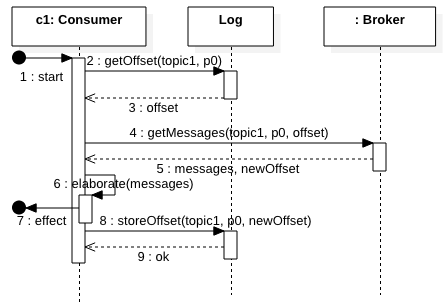
\includegraphics[width=.8\textwidth]{img/kafka-consumer.png}
    \caption{Sequence diagram Kafka consumer.}
\end{figure}

\begin{center}
    \large
    \textcolor{Red2}{\textbf{Kafka architectural tactics}}
\end{center}
There are some tactics used to improve some features of Kafka. In the following section we can see scalability and fault tolerance.

\begin{flushleft}
    \textcolor{Red2}{\textbf{Improve Scalability}}
\end{flushleft}
By \textbf{creating multiple partitions and multiple brokers}, we can create the ability to distribute producers/consumers to different partitions handled by different brokers. We can also \textbf{scale the operations} because Kafka supports the \textbf{creation of clusters of brokers}. Consider that each cluster contains up to a hundred brokers capable of handling trillions of messages per day.

\begin{flushleft}
    \textcolor{Red2}{\textbf{Improve Fault Tolerance}}
\end{flushleft}
By \textbf{creating partitions}, we use the \textbf{persistence} of the partitions. \textbf{Replication} also reduces the risk of data loss. Finally, cluster management takes care of restarting brokers and setting leaders as needed.